\section{Integración numérica}
En diferentes aplicaciones de ingeniería y física es frecuente encontrarse con la necesidad de calcular numéricamente la integral de una función, ya sea que 
esta se tiene definida de manera explícita y su antiderivada no lo es, o en el caso de datos experimentales, cuando la función se encuentra definida de manera 
discreta.  En esta sección revisaremos algunas técnicas simples para abordar el problema de integración numérica de funciones. Inicialmente se revisará (a manera de repaso) la regla extendida del trapecio, la cual es  útil en el caso de funciones definidas. Posteriormente se considerará el caso de una función definida en términos de datos experimentales. Ambos problemas se abordarán para el caso de funciones de una sola variable y posteriormente estos métodos se extenderán al caso de dominios de integración bidimensionales. En la última parte de la sección se abordarán las denominadas formulas Gaussianas, las cuales resultan ser altamente poderosas y versátiles. Estas últimas son de uso común en métodos de elementos finitos y de elementos de frontera.

\subsection{Planteamiento del problema}
En el caso mas general estamos interesados en calcular numericamente integrales de la forma general

\begin{equation}
I\;=\iiint f(x,y,z)dV
\label{sample integral 2}
\end{equation}

donde la integral triple representa integración sobre un volumen determiando. De manera analoga al problema de interpolación, el problema de integración numérica también se resuelve a partir de la solución fundamental de integrar una función uni-dimensional. En cualquier caso, el problema de integración numérica se resuelve mediante una aproximación de la integral en términos de una suma ponderada de la forma:

\begin{equation}
\int\limits_a^b f(x) \dd{x}  \approx \sum\limits_{i=1}^n w_i f(x_i)\, ,
\label{eq:quadra}
\end{equation}

A estas formulas se les denomina {\bf cuadraturas}. En general en una cuadratura (o esquema de integración numérica) se evalúa la función $f(x)$ en $n$ puntos de coordenadas $x_i$ y cada valor de la función es ponderado por un factor $w_i$.


Por ejemplo la \cref{tab:ejemplo} muestra las abscisas (puntos de evaluación) y factores de ponderación de una cuadratura en particular. 

\begin{center}
	\begin{tabular}{cc}
		\hline
		$x_i$ & $w_i$ \\
		\hline
		$-0.86113$  & $0.34785$  \\
		$-0.33998$  & $0.65214$  \\
		$ +0.33998$  & $0.65214$  \\
		$ +0.86113$  & $0.34785$  \\
		\hline
	\end{tabular}
	\captionof{table}{Abscisas y factores de ponderación para calcular 
		$\int\limits_{-1}^{+1} f(x) \dd{x}$.}
	\label{tab:ejemplo}
\end{center}

Usando dicha cuadratura evaluaremos la integral 

\[I = \int\limits_{ - 1}^{ + 1} {({x^3} + 4{x^2} - 10)dx}\]

%\begin{equation}
%I = \int\limits_{ - 1}^{ + 1} {({x^3} + 4{x^2} - 10)dx}
%\label{eq:eje}
%\end{equation} 

La evaluación numérica de la integral se reduce entonces a calcular la siguiente suma ponderada:

\begin{align*}
\int\limits_{-1}^{+1} (x^3 + 4 x^2 - 10) \dd{x} \approx 0.34785 \cdot f(-0.86113) + 0.65214 \cdot f(-0.33998) \\
+ 0.34785 \cdot f(0.86113) + 0.65214 \cdot f(0.33998) = -17.3333
\end{align*}


\paragraph*{Ejemplo: Una aplicación en ingeniería civil.}
Supongamos que queremos calcular el área superficial del Valle de Aburrá. Aunque no conocemos una función que describa la topografía del valle de forma analítica, podemos representar la misma como una serie de puntos con coordenadas (latitud, longitud,  altitud) como se presenta en la siguiente figura.
\begin{figure}[H]
	\centering
	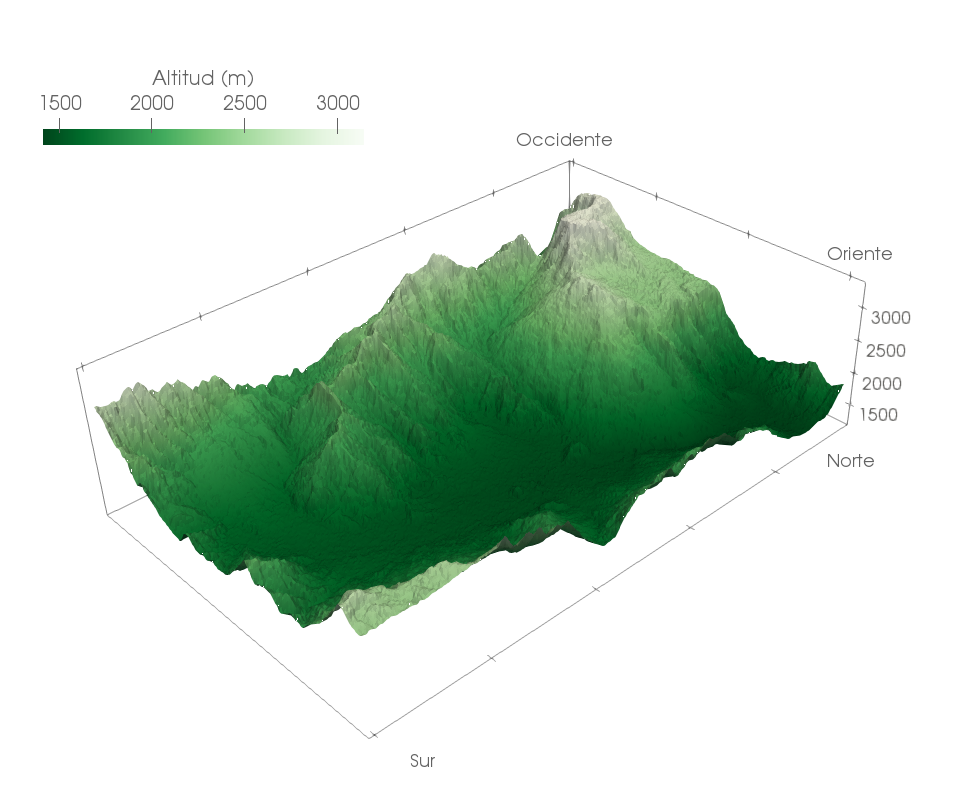
\includegraphics[width=10cm]{valle_aburra.png}
	\caption{Topografía del Valle de Aburrá.}
\end{figure}

Podemos utilizar las técnicas de interpolación vistas anteriormente para calcular la integral de superficie en el valle. Con la siguiente fórmula podríamos calcular el área superficial

\[A = \int\limits_\text{Dominio}{\sqrt{\left(\pdv{f(x, y)}{x}\right)^2 + 
\left(\pdv{f(x, y)}{y}\right)^2 + 1}}\; \dd{x}\dd{y}\, ,\]

en donde las coordenadas \((x, y)\) se corresponden con (longitud, latitud),  
la función \(f(x, y)\) es la altitud para cada uno de los puntos, y la integral 
se hace sobre el dominio sobre el que está definida la superficie.


\subsection{Integración numérica mediante polinomios de interpolación}

La integración numérica se basa fundamentalmente en el ajuste de un polinomio 
de interpolación $p(x)$ a la función dada $f(x)$ a través de $n$ puntos en 
los cuales se conoce o calcula el valor de la función, para luego usar 
$\int_a^b p(x)\dd{x}$ como una aproximación a la integral de $f(x)$. El número 
de evaluaciones de $f(x)$, así como las posiciones de los puntos de evaluación 
determinan que tan buena es la aproximación de $p(x)$ a $f(x)$ y por ende el 
error en la aproximación de la integral.

Concretamente, en los algoritmos de integración numérica se hace la aproximación:
\[\int\limits_a^b f(x) \dd{x} \approx \int\limits_a^b p(x) \dd{x}\, , \]
donde 
\[p(x) = \sum_{i=1}^n L_i(x) f(x_i)\]
siendo ${L_i}(x)$ el polinomio interpolante de Lagrange asociado al punto $x_i$.

Aproximando la función mediante un polinomio de interpolación se tiene que:
\[\int\limits_a^b f(x) \dd{x}  \approx \int\limits_a^b \sum_{i=1}^n 
L_i(x)f(x_i) \dd{x}  
\equiv \sum_{i=1}^n f(x_i)\int\limits_a^b L_i(x) \dd{x} \, , \]
la cual es equivalente a la \cref{eq:quadra} y en la cual se identifica que los 
factores de ponderación están dados por:
\begin{equation}
w_i \equiv \int\limits_a^b L_i(x) \dd{x} \, . 
\label{eq:pesos}
\end{equation}

Este tipo de esquemas se divide en métodos de Newton-Cotes y en cuadraturas 
Gaussianas. En el primer caso el intervalo de integración se divide en $n - 1$ 
sub-intervalos iguales (delimitados por abscisas equidistantes) de tamaño 
$(b-a)/(n - 1)$. En el segundo caso se dejan como parámetro de ajuste tanto la 
localización de los puntos de evaluación como los factores de ponderación, 
resultando en un esquema más versátil. A continuación se discuten ambas 
estrategias.


\subsection{Regla del trapecio}
Considere el caso particular en el que se tienen 2 puntos (1 intervalo de 
integración). El tamaño del intervalo en este caso corresponde a 
$h = b - a$ y el polinomio de interpolación de $f(x)$ está dado por:
\[p(x) = L_1(x) f_1 + L_2(x) f_2 \equiv L_1(x) f(a) + L_2(x) f(b)\, .\]

Los polinomios interpolantes en este caso son:
\begin{align*}
  &L_1(x) = \frac{(x - x_2)}{(x_1 - x_2)} \equiv  - \frac{1}{h}(x - b)\, \\
  &L_2(x) = \frac{(x - x_0)}{(x_2 - x_1)} \equiv \frac{1}{h}(x - a)\, .
\end{align*}

Reemplazando en \eqref{eq:pesos} se tiene que:
\begin{align*}
  &w_1 =  - \frac{1}{h}\int\limits_a^b (x - b) \dd{x}  \equiv \frac{h}{2}\, ,\\
  &w_2 =  + \frac{1}{h}\int\limits_a^b (x - a) \dd{x}  \equiv \frac{h}{2}\, ,
\end{align*}
de donde:
\[I = w_1 f_1 + w_2 f_2 \equiv \frac{h}{2}\left[f(a) + f(b)\right]\, .\]

Y, finalmente,
\begin{equation}
  \int\limits_a^b f(x) \dd{x} \approx \frac{h}{2}[ f(a) + f(b)]\, .
  \label{eq:trapecio}
\end{equation}

\subsubsection*{Ejemplo}
Calcular
\[I=\int\limits_{-1}^{+1} (x^3 + 4 x^2 - 10) \dd{x}\, ,\]
usando la regla del trapecio.

En este caso \(h=2.0\), luego:
\[I = f(-1) + f(1) \equiv  -7 - 5 = -12\]

Considere nuevamente la regla del trapecio dada en la \cref{eq:trapecio}. 
Supongamos un intervalo de integración con límites $x_1 = a$ y $x_n = b$ 
y en el cual se conocen en total $n$ valores de una función $f(x)$ (ver 
\cref{fig:test})
\begin{figure}[H]
\centering
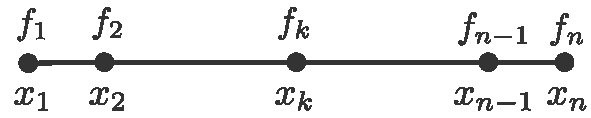
\includegraphics[width=10cm]{testline.pdf}
\caption{Intervalo de integración extendido con puntos de muestreo entre $x_1$ 
y $x_n$.}
\label{fig:test}
\end{figure}

Aplicando la \cref{eq:trapecio} $n - 1$ veces para hacer la integración en los 
sub-intervalos $(x_1, x_2),\, (x_2,x_3),\cdots,\, (x_{n-1},x_{n})$ y sumando 
los resultados se obtiene:
\begin{equation}
\int\limits_a^b f(x) \dd{x} = h\left[\frac{1}{2}f_1 + f_2 + f_3 + f_4 + \cdots 
+ f_{n-1} + \frac{1}{2}f_n \right]  + O\left[\frac{(b - a)^3 f''}{n^2} \right]
\label{eq:trap_comp}
\end{equation}
la cual es válida para calcular la integral usando los $n$ puntos $x_1,\, 
x_2,\cdots, x_{n- 1 }, x_{n}$. En esta expresión $h$ es la separación entre 
puntos.

En el apendice se describe la función {\bf trapz} (correspondiente a la 
\cref{eq:trap_comp}) la cual integra una función {\bf $f(x)$} entre los puntos $a$ y $b$. La 
rutina realiza la transformación del rango $[a,b]$ al ficticio dado por $[-1, 
+1]$. Usando esta función en el calculo de la integral del ejemplo antrior se tiene la siguiente salida:

\begin{verbatim}
Approximation for 1 subdivisions: -12.000000
Approximation for 2 subdivisions: -16.000000
Approximation for 3 subdivisions: -16.740741
Approximation for 4 subdivisions: -17.000000
Approximation for 5 subdivisions: -17.120000
Approximation for 6 subdivisions: -17.185185
Approximation for 7 subdivisions: -17.224490
Approximation for 8 subdivisions: -17.250000
Approximation for 9 subdivisions: -17.267490
Analytic integral: -17.333333
\end{verbatim}

\begin{tcolorbox}
En las cuadraturas de Newton-Cotes, como la regla del trapecio, los puntos de evaluación de la función son equidistantes. En las cuadraturas Gaussianas los puntos de evaluación no son equidistantes sino que estan localizados en ciertas posiciones de manera que la cuadratura sea lo mas eficiente posible.
\end{tcolorbox}



\subsection{Cuadraturas Gaussianas}
En la cuadratura correspondiente a la regla extendida del trapecio escrita de la forma
\begin{equation}
\int\limits_a^b f(x) \dd{x} \approx \sum\limits_{i=1}^{n} w_i f(x_i)\, ,
\label{quadra2}
\end{equation}
los puntos de evaluación se encuentran espaciados de manera equidistante. En 
las cuadraturas Gaussianas se dejan como parámetros por ajustar los factores de 
ponderación $w_i$ y también la localización de los puntos de evaluación $x_i$. 
Como resultado, ahora se dispone de $2n$ parámetros para ajustar y
así resolver el problema de calcular la integral de $f(x)$ entre $x=a$ y $x=b$ 
con la máxima precisión y el mínimo número de operaciones. Este 
tipo de cuadraturas proveen mayor precisión que las del tipo Newton-Cotes (como 
las del trapecio) cuando la función a integrar es apropiadamente representable 
mediante un polinomio. Considerando lo anterior se tiene que por medio de una 
cuadratura Gaussiana es posible integrar funciones expresables como:
\[\int\limits_a^b w(x) f(x) \dd{x}  \approx \sum\limits_{I = 1}^{n} w_i 
f(x_i)\, . \]

La factorización \(w(x) f(x)\) es útil ya que permite expresar una función como 
el producto de un polinomio $f(x)$ por una función conocida $w(x)$. Esta última 
puede seleccionarse para remover singularidades integrables de la integral.

%Considere a manera de ejemplo la integral de Gauss-Chebyshev:
%\[\int\limits_{-1}^1 \frac{e^{-cx^2}}{\sqrt {1 - x^2}} \dd{x} \equiv 
%\int\limits_{-1}^1 \frac{1}{\sqrt{1 - x^2} } e^{ -cx^2}\dd{x}\]
%donde
%\[w(x) = \frac{1}{\sqrt{1 - x^2}}\]
%mientras que: 
%\[f(x) = e^{ -cx^2}\, .\]
%
%Haciendo
%\[g(x) = w(x)f(x)\]
%y
%\[v_i = \frac{w_i}{w(x_i)}\, ,\]
%se tiene que:
%\begin{equation}
%  \int\limits_{-1}^{+1} g(x)\dd{x}  \approx \sum\limits_{i = 1}^{n} v_i 
%  g(x_i)\, .
%  \label{eq:gauss}
%\end{equation}

Las diferentes cuadraturas Gaussianas se encuentran especificadas en 
términos de una tabla de valores de abscisas de los puntos de integración (o de 
evaluación de la función a integrar) y sus correspondientes factores de 
ponderación (también denominados pesos). Por ejemplo la \cref{tab:ejemplo2} 
presenta las abscisas y factores de ponderación para una cuadratura de 4 puntos.
\begin{center}
\begin{tabular}{cc}
  \hline
  $x_i$ & $w_i$ \\
  \hline 
  $-0.86113$  & $0.34785$  \\
  $-0.33998$  & $0.65214$  \\
  $ +0.33998$  & $0.65214$  \\
  $ +0.86113$  & $0.34785$  \\
  \hline
\end{tabular}
\captionof{table}{Abscisas y factores de ponderación para calcular 
$\int\limits_{-1}^{+1} f(x) \dd{x}$}
\label{tab:ejemplo2}
\end{center}

Para facilitar la codificación de las cuadraturas y permitir cálculos 
generales, es común considerar el intervalo de integración canónico 
$[-1.0,+1.0]$, por lo que es necesario transformar la integral (incluyendo la 
función, los límites y el diferencial) a dicho intervalo como se 
discute en la \cref{sec:isopar}. La \cref{fig:quagauss} esquematiza este 
intervalo y los correspondientes puntos de integración (denotados por los 
círculos blancos). En la siguiente sección se desarrolla un ejemplo completo de 
evaluación de una integral por medio de una cuadratura Gaussiana tras realizar 
la transformación al dominio canónico.
\begin{figure}[H]
\centering
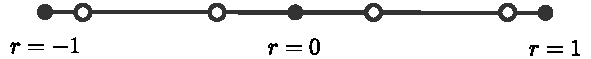
\includegraphics[width=10cm]{quagauss.pdf}
\caption{Esquematización de una cuadratura Gaussiana en el intervalo canónico 
$[-1.0,1.0]$.}
\label{fig:quagauss}
\end{figure}


\begin{tcolorbox}
En las cuadraturas Gaussianas los puntos de evaluación se encuentran especificados en el intervalo $[-1.0 , 1.0]$ el cual se denomina el espacio canonico. Es común denotar el espacio canonico mediante la variable $r$, de manera que para integrar una función en el intervalo $x \in [a , b]$ primero es necesario transformas la función y el dominio de integración al intervalo canonico $r \in [-1.0, 1.0].$
\end{tcolorbox}


\paragraph*{Ejemplo de derivación de una cuadratura Gaussiana.}
Revisemos el proceso de derivación de una cuadratura Gaussiana. Para esto supongamos que queremos formular una cuadratura correspondiente a $n=2$, o equivalentemente una cuadratura de 2 puntos , asumiendo que el intervalo de integración es $[a,b]=[-1,+1]$ de tal forma que coincida con el del intervalo canonico. Queremos entonces determinar los valores de los factores de ponderación $w_1$ y $w_2$ así como la localización de los puntos de evaluación $x_1$ y $x_2$ de manera que la cuadratura podamos integrar de manera exacta una función correspondiente a un polinomio de grado $3$ que tiene la forma general:

\[f(x) = a_0 + a_1 x + a_2 x^2 + a_3 x^3\, .\]

En otras palabras, queremos encontrar valores apropiados de $w_1$, $w_2$, $x_1$ y $x_2$ tales que se satisfaga:

\[I = \int\limits_{-1}^{+1} f(x)\dd{x}  \equiv w_1 f(x_1) + w_2 f(x_2)\, .\]

Usando $f(x)$ en $I$ y planteando la integral para cada termino se obtiene:
\[I = \int\limits_{-1}^{+1} a_0 \dd{x}  + \int\limits_{-1}^{+1} a_1 x\dd{x}  + \int\limits_{-1}^{+1} a_2 x^2 \dd{x}  + \int\limits_{-1}^{+1} a_3 x^3 \dd{x} \]

donde identificamos un término constante, un término de orden 1, un término cuadratico y un término de orden3. Para que la cuadratura sea exacta cada uno de estos términos debe poder ser integrado de manera exacta. Usando esta condición se tiene:

\begin{align*}
  &\intL_{-1}^{+1} \dd{x}  = 2 = w_1 \cdot 1 + w_2 \cdot 1\, ,\\
  &\intL_{-1}^{+1} x\dd{x}  = 0 = w_1 \cdot x_1 + w_2 \cdot x_2\, ,\\
  &\intL_{-1}^{+1} x^2 \dd{x}  = \frac{2}{3} = w_1 \cdot x_1^2 + w_2 \cdot 
  x_2^2\, ,\\
  &\intL_{-1}^{+1} x^3 \dd{x}  = 0 = w_1 \cdot x_1^3 + w_2 \cdot x_2^3\, .
\end{align*}


Se tiene un sistema de  ecuaciones en 4 incognitas correspondientes a los factores de ponderación $w_1$, $w_2$ y los puntos de evaluación $x_1$ y $x_2$. Resolviendo el sistema se tiene que $w_1 = 1$, 
$w_2 = 1$, $x_1 =-\sqrt{3}/3$ y $x_2 =  + \sqrt{3}/3$. Usando este resultado en la expresón de la cuadratura $I$ se tiene:

\[I = \int\limits_{-1}^{+1} f(x) \dd{x}  \approx 1.0 \cdot f(-\sqrt{3}/3) + 1.0 
\cdot f(+\sqrt{3}/3).\]

Claramente esta cuadratura es exacta si se trata de integrar funciones polinómicas de orden 3 o menor. Notese que la posibilidad de ajustar 4 paramétros $(w_1, w_2, x_1, x_2)$ permitió integrar de manera exacta una función de orden $3$. Mas adelante se demostrará que una cuadratura Gaussiana de orden $n$ permite integrar de manera exacta funciones de orden $2n-1$. Notese también que la localización de los puntos de integración $x_1$ y $x_2$ es simetrica con respecto a $x=0$: Mas aún, en este caso se satisface que $x_1 = - x_2$.

La idea de la cuadratura Gaussiana es extendible a polinomios de grado mayor, 
pero se requiere de un método efectivo para determinar los factores de
ponderación y abscisas de evaluación. En la siguiente sección se presentará un 
método aplicable a polinomios de orden $2n$, en el que se saca provecho de la 
propiedad de ortogonalidad de ciertos polinomios especiales.

\paragraph*{Polinomios ortogonales}
Dos polinomios $P(x)$ y $Q(x)$ donde $P(x) \ne Q(x)$ son ortogonales si:

\[\int\limits_a^b {P(x)Q(x)} dx = 0.\]
Particularmente, los polinomios de Legendre definidos por
\[P_n(x) = \frac{1}{2^n n!}\dv[n]{x} [(x^2 - 1)^n]\]
y los cuales son solución a la ecuación:
\[(1 - {x^2}) y'' - 2x y' + n(n + 1)y = 0\]
en el intervalo $[-1,+1]$ satisfacen la siguiente condición de ortogonalidad
\[\int\limits_{ - 1}^{ + 1} {{Q_i}(x)} {P_j}(x)\dd{x} = 0\, ,\]
donde  ${{Q_i}(x)}$ es cualquier función polinomial de grado $i$ menor que $j$.

Además de la propiedad de ortogonalidad los polinomios de Legendre tiene raíces 
en el intervalo $(-1.0, 1.0)$ las cuales son diferentes y simétricas con 
respecto a cero. Como se demuestra en el siguiente teorema esta ultima propiedad hace que estas raíces puedan ser útiles 
para producir una cuadratura que sea exacta para integrar cualquier función 
polinomial de grado menor que $2n$. Por ejemplo, el segundo polinomio de 
Legendre dado por:
\[{P_2}(x) = {x^2} - \frac{1}{3}\]
tiene como raíces $x_1 =  - \frac{\sqrt{3}}{3}$ y $x_2 =  +\frac{\sqrt{3}}{3}$ 
los cuales corresponden a los puntos de integración para la cuadratura
exacta de grado 3 encontrada en el ejemplo anterior.

\paragraph*{Teorema}
Sean $\left\{ x_1, x_2,\cdots, x_n \right\}$ las raíces del polinomio de 
Legendre $P_n(x)$ de grado $n$; sea
\[w_i = \int\limits_{-1}^{+1} \prod\limits_{j=1}^n \frac{x - x_j}{x_i - x_j} 
\dd{x}\, , \]
y sea $f(x)$ una función polinomial cualquiera de grado menor que $2n$, entonces:
\begin{equation}
  I = \int\limits_{-1}^{+1} f(x)\dd{x}  = \sum\limits_{i=1}^n w_i f(x_i)\, .
  \label{eq:Legendre}
\end{equation}


\paragraph*{Demostración}

\begin{enumerate}
\item Si $f(x)$ es de grado menor que $n$ entonces claramente es representable 
en términos de polinomios de Lagrange con lo cual se satisface de manera 
automática la condición \cref{eq:Legendre}.

\item Si $f(x)$ es de grado menor que $2n$ entonces es representable como:
\[f(x) = Q(x){P_n}(x) + R(x)\]
donde $Q(x)$ es el cociente de $f(x)/{P_n}(x)$ y de grado $n-1$ (o menor) y $R(x)$ es el residuo y de grado menor que $n$. Integrando esta representación de $f(x)$ se tiene:
\[\int\limits_{-1}^{+1} Q(x) P_n(x) \dd{x}  + \int\limits_{-1}^{+1} R(x) \dd{x}\, , \]
la cual se reduce a:
\[I = \int\limits_{ -1}^{ +1} f(x) \dd{x}  = \int\limits_{ -1}^{ +1} R(x)\ \dd{x}\, , \]
tras usar la propiedad de ortogonalidad entre $Q(x)$ y $P_n (x)$. Ahora, retomando la expresión:
\[f(x) = Q(x){P_n}(x) + R(x)\]
si esta es evaluada en las raíces de los polinomios de Legendre se tiene que:
\[f(x_i) = R(x_i)\]
con lo cual queda completa la demostración.

\end{enumerate}

\subsection{Transformación del dominio de solución}\label{sec:isopar}
La construcción de tablas con las coordenadas y factores de ponderación de las diferentes cuadraturas y su programación en el computador se facilita si estas se especifican para un rango fijo. Por diversas conveniencias matemáticas, es común usar como 
intervalo general el dado por $[-1, 1]$ denominado previamente como el intervalo canonico y descrito mediante una variable independiente, comunmente denotada como $r$. Se tiene entonces que el espacio de la variable independiente correspondiente a $x \in [a , b]$ se transforma el espacio canonico dado por $r \in [-1.0 , 1.0]$. Note que esta transformación también implica una transformación de la función $f(x)$ en el espacio de $x$ a su respresentación en el espacio de $r$.

Es necesario entonces reescribir la integral de $f(x)$ en el rango comprendido entre $x=a$ y $x=b$ a una integral en el espacio canonico de acuerdo con:
\begin{equation}
\int\limits_a^b f(x) \dd{x} \equiv \int\limits_{-1}^{+1} F(r) \dd{r}\, . 
\label{eq:trans}
\end{equation}


La transformación \ref{eq:trans} se describe en la \cref{fig:map} y en la cual la flecha curva esquematiza la transformación entre los 2 espacios a saber, el espacio representado mediante la variable independiente $x$ y 
comprendido entre $x=a$ y $x=b$ y el espacio canonico descrito mediante la variable  $r$ y comprendido entre $r=-1$ y  $r=1$.

\begin{figure}[H]
\centering
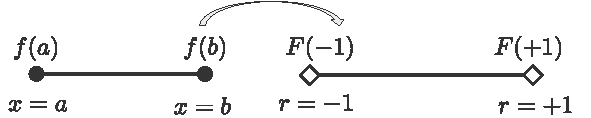
\includegraphics[width=10cm]{transformacion.pdf}
\caption{Transformación del rango de integración $[a,b]$ al intervalo canónico 
$[-1.0,+1.0].$}
\label{fig:map}
\end{figure}

La transformación espacial puede indicarse matemáticamente como:
\begin{align*}
  x = x(r)\, ,
  r = r(x)\, ,
\end{align*}
y en la cual $x(r)$ y $r(x)$ denotan relaciones funcionales entre los 2 espacios. Es evidente que independiente de la forma de la relación funcional esta minimamente debe satisfacer las condiciones $x(-1.0)=a$ y $x(+1)=b$. Por ejemplo, una relación relación funcional válida puede encontrarse tras asumir que ambos espacios están relacionados mediante un polinomio de interpolación de Lagrange de primer grado construido como:

\[x(r) = L_1(r) x(r_1) + L_2(r) x(r_2)\, .\]

Usando los correspondientes polinomios interpolantes:

\begin{align*}
  &L_1(r) = \frac{r - r_2}{r_1 - r_2} \equiv \frac{1}{2}(1 - r)\, ,\\
  &L_2(r) = \frac{r - r_1}{r_2 - r_1} \equiv \frac{1}{2}(1 + r)\, ,
\end{align*}

en la expresión para $x(r)$ se tiene que:

\[x(r) = \frac{1}{2}(a + b) + \frac{r}{2}(b - a).\]

Continuando con la transformación es claro que también es necesario reescribir $f(x)$ en términos de  $r$  de acuerdo con:

\[f = f(x) \equiv f[x(r)] = \hat F(r)\, .\]

Finalmente, para completar la transformación es necesario transformar el diferencial de "espacio físico", es decir $dx$ a su correspondente diferencial en el espacio canonico $dr$. Procediendo directamente desde la transformación en términos de los polinomios de Lagrange se tiene que:

\[\dv{x}{r}  = \dv{L_1(r)}{r} x(r_1) + \dv{L_2(r)}{r} x(r_2) \equiv 
\frac{1}{2}(b - a)\, ,\]

y por lo tanto

\[\dv{x}{r} = \frac{1}{2}(b - a)\]

lo cual permite escribir finalmente la integral en el dominio ficticio comprendido entre $[-1, +1]$ de acuerdo con:

\[\int\limits_a^b f(x) \dd{x} \equiv \int\limits_{-1}^{+1} \hat F(r)\frac{h}{2} 
\dd{r} \equiv \int\limits_{-1}^{+1} F(r) \dd{r}\, , \]

y donde $h = \frac{1}{2}(b - a).$

\subsubsection*{Ejemplo}

Usar una cuadratura Gaussiana de 2 puntos (ver \cref{ejemplo3}) para evaluar la integral:
\[I = \int\limits_0^3 (2^x - x) \dd{x}\, . \]

\begin{center}
\begin{tabular}{cc}
  \hline
  $x^I$ & $w^I$ \\
  \hline 
  $-0.5773503$  & $1.000000$  \\
  $+0.5773503$  & $1.000000$  \\
  \hline
\end{tabular}
\captionof{table}{Abscisas y factores de ponderación para calcular $\int_{-1}^{+1} f(r) \dd{r}$}
\label{ejemplo3}
\end{center}

Para realizar la integración usando la cuadratura Gaussiana de 2 puntos dada en la \cref{ejemplo3} es necesario transformar el rango de integración y el integrando de la función al espacio correspondiente al intervalo $[-1.0,+1.0]$. Esta transformación está dada por:
\[x(r) = \frac{3}{2} + \frac{3}{2}r\]
mientras que los elementos diferenciales satisfacen
\[\dd{x} = \frac{3}{2}\dd{r}\, .\]

Para transformar la función usamos
\[\hat f(r) = f[x(r)] \equiv f\left( \frac{3}{2} + \frac{3}{2}r \right)\, ,\]
de donde se tiene que
\[I = \int\limits_0^3 (2^x - x) \dd{x} = \int\limits_{-1.0}^{+1.0} \left[ 2^{\frac{3}{2}(1 + r)} - \frac{3}{2}(1 + r) \right] \frac{3}{2} \dd{r} \, ,\]
y evaluando,
\begin{align*}
  I &= \sum\limits_{i=1}^2 w_i\left[ 2^{\frac{3}{2}(1 + r_i)} - \frac{3}{2}(1 + 
  r_i) \right]\frac{3}{2}\\
  &= 1.0 \cdot (1.37678967978) + 1.0 \cdot (4.18374583924)\\
  &= 5.56053551
\end{align*}

En el apendice se presenta a manera de función la implementación en Python de la cuadratura Gaussiana de 2 puntos. La rutina hace uso  de la función {\bf gauss1d} para integrar la función definida en {\bf $f(x)$}. La rutina realiza la transformación de $[a,b]$ a $[-1, +1]$.

%\pagebreak
%\begin{minted}[mathescape,
%	gobble=4,
%	frame=lines,
%	framesep=2mm]{python} 
%    import numpy as np
%    from scipy.special import roots_legendre # Gauss points and weights
%    from sympy import symbols, integrate
%    
%    
%    def gauss1d(fun, x0, x1, n):
%    """Gauss quadrature in 1D
%    
%    Parameters
%    ----------
%    fun : callable
%        Function to integrate.
%    x0 : float
%        Initial point for the integration interval.
%    x1 : float
%        End point for the integration interval.
%    n : int
%        Number of points to take in the interval.
%    
%    Returns
%    -------
%    inte : float
%         Approximation of the integral
%    
%    """
%    xi, wi = roots_legendre(n)
%    inte = 0
%    h = 0.5 * (x1 - x0)
%    xm = 0.5 * (x0 + x1)
%    for cont in range(n):
%        inte = inte + h * fun(h * xi[cont] + xm) * wi[cont]
%    return inte
%
%    fun = lambda x: x**3 + 4*x**2 - 10
%    gauss_inte = gauss1d(fun, -1, 1, 4)
%    x  = symbols('x')
%    analytic_inte = integrate(fun(x) , (x , -1 , 1))
%    print("Analytic integral: {:.6f}".format(float(analytic_inte)))
%    print("Gauss quadrature: {:.6f}".format(gauss_inte))
%\end{minted}

Si ejecutamos la rutina, obtenemos el siguiente resultado:
\begin{verbatim}
Analytic integral: -17.333333
Gauss quadrature: -17.333333
\end{verbatim}

\subsection{Extensión a dominios en 2D}
En varias aplicaciones de ingeniería es necesario el calculo de integrales sobre dominios bi-dimensionales, posiblemente con geométrias arbitrarias. En esta sección se generaliza la idea de la cuadratura numérica presentada en los numerales anteriores para funciones de 1 sola variable independiente al caso de funciones de varias variables. En particular, acá ausmimos que las variables independientes representan coordenadas $x , y$ de un espacio cartesiano.

En la \cref{fig:rieman} se esquematiza un dominio en 2-dimensiones (línea negra continua) denotado como $R$ y sobre el cual se desea calcular una integral de la forma
\[I = \iint\limits_R f(x,y) \dd{A}\, . \]

Para proceder con el cálculo el dominio se ha dividido en $N$ subdominios 
rectangulares (líneas negras punteadas) de manera que un subdominio típico 
tiene dimensiones $\Delta {x_i} \times \Delta {y_i}$.

\begin{figure}[H]
\centering
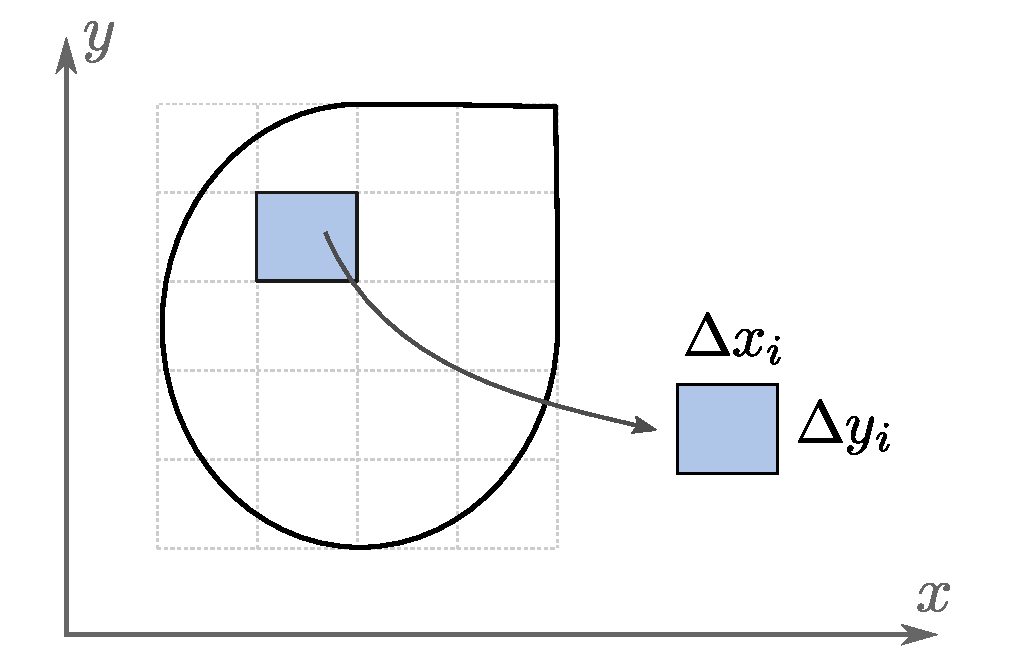
\includegraphics[width=10cm]{riemann.pdf}
\caption{Partición de Riemman para un dominio plano.}
\label{fig:rieman}
\end{figure}

Definiendo

\[p = \max\{ \Delta {x_i}, \Delta {y_i} \}\, ,\]

como la norma de la partición, se tiene, de acuerdo a la definición de una integral como una suma de Riemann, que:

\[I = \iint\limits_R  f(x,y) \dd{A}  \equiv \lim_{p \to 0} \sum_{j=1}^N f(x_j,y_j) \Delta x_j \Delta y_j\, .\]

Ahora, tomando cada uno de los límites en la dirección $x$ y $y$ por separado permite identificar 2 procesos de integración de tal forma que la integral sobre $R$ se reduce a la integral doble dada por:

\[I = \iint f(x,y) \dd{x}\dd{y}\, . \]

Para identificar los límites de integración considere la \cref{fig:dirx}. En esta se muestra un dominio de integración rectangular (en sombreado azul) cuyo lado mayor es paralelo a la dirección $x$ y con altura media correspondiente a un valor constante $y$. Los lados menores del rectángulo tienen abscisas $x_1(y)$ y $x_2(y)$ respectivamente.
\begin{figure}[H]
\centering
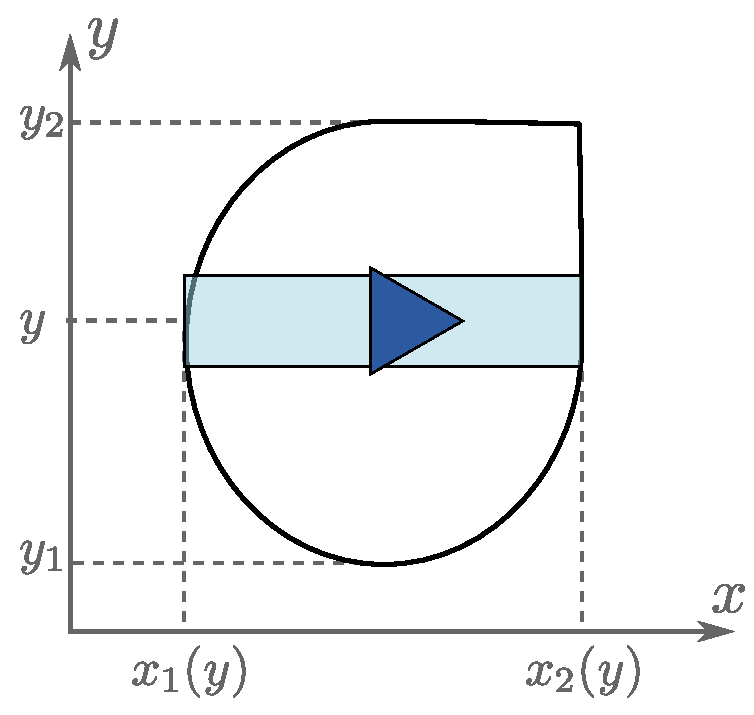
\includegraphics[width=8cm]{inte_dirx.pdf}
\caption{Integración en la dirección x.}
\label{fig:dirx}
\end{figure}

Claramente se tiene que para el valor de $y$ constante la contribución a la integral $I$ sobre la región $R$ del rectángulo acotado por ${x_1}(y)$ y ${x_2}(y)$ esta dada por:

\[\int\limits_{x_1(y)}^{x_2(y)} f(x,y) \dd{x}\, ,\]

de forma que el cálculo de la integral sobre la totalidad de la región $R$ se 
completa repitiendo el proceso para valores de $y$ constantes variando entre 
$y_1$ y $y_2$ y dando la integral total como:

\begin{equation}
  I = \int\limits_{y_1}^{y_2} \left\{ \int\limits_{x_1(y)}^{x_2(y)} f(x,y) \dd{x}  \right\} \dd{y}
  \label{iterada}
\end{equation}


Para dar mayor claridad a la \cref{iterada}, nótese que la integral interna puede escribirse como una función de $y$

\[F(y) = \int\limits_{x_1(y)}^{x_2(y)} f(x,y) \dd{x}\, , \]
y la integral externa como
\[I = \int\limits_{y_1}^{y_2} F(y) \dd{y}\, . \]

Notese que el calculo de $I$ se ha reducido a 2 integrales uni-dimensionales y en consecuencia el proceso puede resolverse por medio de las cuadraturas uni-dimensionales ya discutidas. En este caso la función mas interna $F(y)$ resulta de integrar solo la variación en $x$ y posteriormente la integral $I$ resulta de integrar la variación en $y$. Alternativamente (ver \cref{fig:diry}) también es posible definir

\[H(x) = \int\limits_{y_1(x)}^{y_2(x)} f(x,y) \dd{y} \]

de manera que la integral completa $I$ queda definida por

\[I = \int\limits_{x_1}^{x_2} H(x) \dd{x}. \]

\begin{figure}[H]
\centering
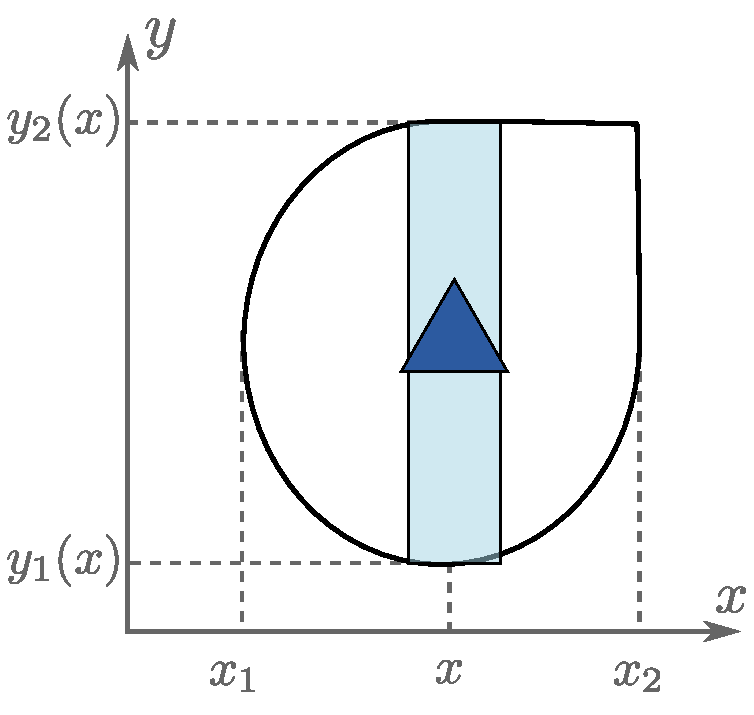
\includegraphics[width=8cm]{inte_diry.pdf}
\caption{Integración en la dirección y.}
\label{fig:diry}
\end{figure}


\subsubsection*{Ejemplo}

Considere la región (o dominio) triangular de la \cref{fig:ejeint}.
\begin{figure}[h]
	\centering
	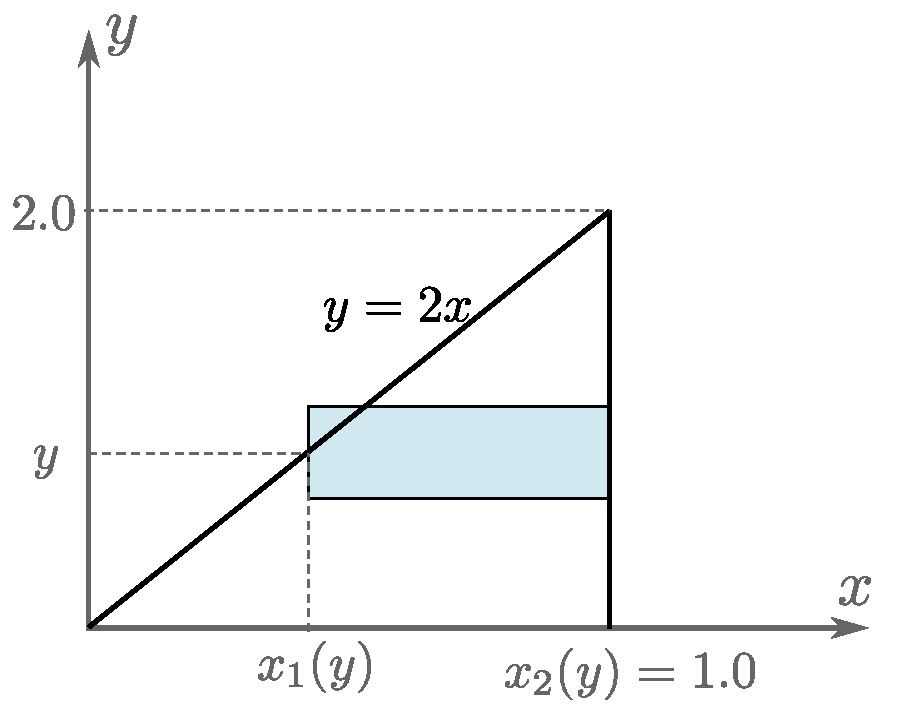
\includegraphics[width=8cm]{ejeint.pdf}
	\caption{Integración en la dirección x sobre la región triangular $R$.}
	\label{fig:ejeint}
\end{figure}

Utilice el concepto de integrales iteradas discutido anteriormente para 
determinar la integral de la función
\[f(x,y)=x y^2\]
sobre la región $R$ de la figura.

La integral sobre $R$ esta dada por
\[I = \iint f(x,y) \dd{A}\]
donde $\dd{A}$ representa un elemento diferencial de superficie. Supongamos que 
tomaremos rectángulos paralelos al eje $x$ de manera que para valores 
constantes de $y$ se tiene:
\[x_1(y) = \frac{y}{2}\]
y
\[x_2(y) = 1\]
y por lo tanto se tiene que:
\[F(y) = \int\limits_{x_1(y)}^{1.0} x y^2 \dd{x}  \equiv \int\limits_{y/2}^{1.0} x y^2 \dd{x}\, , \]
luego
\[F(y) = \left[ \frac{1}{2} x^2 y^2 \right]_{y/2}^{1.0} \equiv \frac{1}{2} y^2 
- \frac{1}{8}  y^4\, .\]
Identificando ahora los limites inferior y superior en la dirección $y$ como 
${y_1} = 0$ y ${y_2} = 2$ es posible integrar la dependencia en $y$ de acuerdo 
con:
\[I = \int\limits_0^{2.0} F(y) \dd{y}  \equiv \int\limits_0^{2.0} 
\left(\frac{1}{2}y^2 - \frac{1}{8} y^4\right) \dd{y}  \equiv \frac{8}{15}\, .\]


% respectivamente y las funciones ${{x_1}(y)}$ y ${{x_2}(y)}$  como:
%\[x_1(y) = \frac{y}{2}\]
%y
%\[x_2(y) = 1\]
%se tiene que:
%\[F(y) = \int\limits_{x_1(y)}^{1.0} x y^2 \dd{x}  \equiv \int\limits_{y/2}^{1.0} x y^2 \dd{x}\, , \]
%luego
%\[F(y) = \left[ \frac{1}{2} x^2 y^2 \right]_{y/2}^{1.0} \equiv \frac{1}{2} y^2 
%- \frac{1}{8}  y^4\, .\]
%Usando esta función para integrar en $y$ se llega a
%\[I = \int\limits_0^{2.0} F(y) \dd{y}  \equiv \int\limits_0^{2.0} 
%\left(\frac{1}{2}y^2 - \frac{1}{8} y^4\right) \dd{y}  \equiv \frac{8}{15}\, .\]

Procediendo de manera alternativa (ver \cref{fig:ejeinty}) es posible escribir:
\[H(x) = \int\limits_{y_1(x)}^{y_2(x)} x y^2 \dd{y} \]
y
\[I = \int\limits_{x_1}^{x_2} H(x) \dd{x}\, . \]

\begin{figure}[H]
\centering
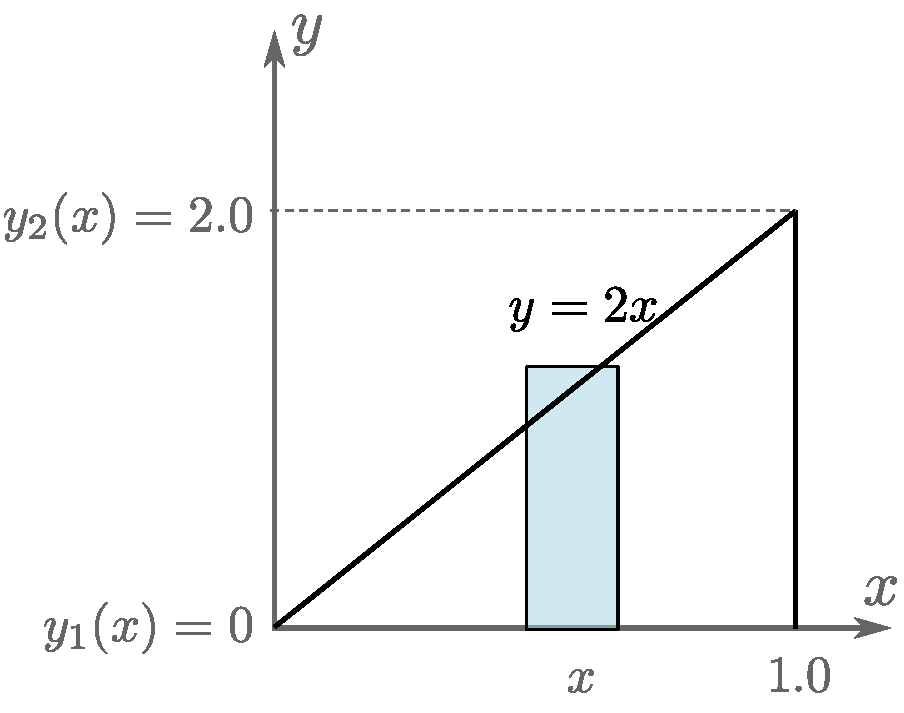
\includegraphics[width=8cm]{ejeinty.pdf}
\caption{Integración en la dirección y sobre la región triangular $R$.}
\label{fig:ejeinty}
\end{figure}
donde:
\[{y_1}(x) = 0\]
\[{y_2}(x) = 2x\]
luego
\[H(x) = \int\limits_0^{2x} {x{y^2}dy}  \equiv \left. {\frac{1}{3}x{y^3}} \right|_0^{2x} \equiv \frac{8}{3}{x^4}\]
de manera que la integral se reduce a:
\[I = \int\limits_0^{1.0} {\frac{8}{3}{x^4}dx}  \equiv \frac{8}{{15}}.\]

En el apéndice se presenta una rutina con la correspondiente implementación en 
Python del esquema de integrales iteradas. Esta permite calcular integrales 
sobre regiones rectangulares. Por ejemplo si se calcula la siguiente integral

\[\int\limits_0^2\int\limits_0^2 [3xy^2 - x^3] \dd{x}\dd{y} = 8\, , \]

usando la rutina código se obtiene el siguiente resultado:

\begin{verbatim}
Gauss quadrature: 8.000000
\end{verbatim}

\newpage
\subsubsection{Ejercicios}
\begin{enumerate}

\item \label{punto01} Calcule la integral de la función
\[f(x,y)=4x^2+3xy+y^2\]
sobre los dominios planos mostrados en las figuras
\begin{figure}[H]
	\centering
	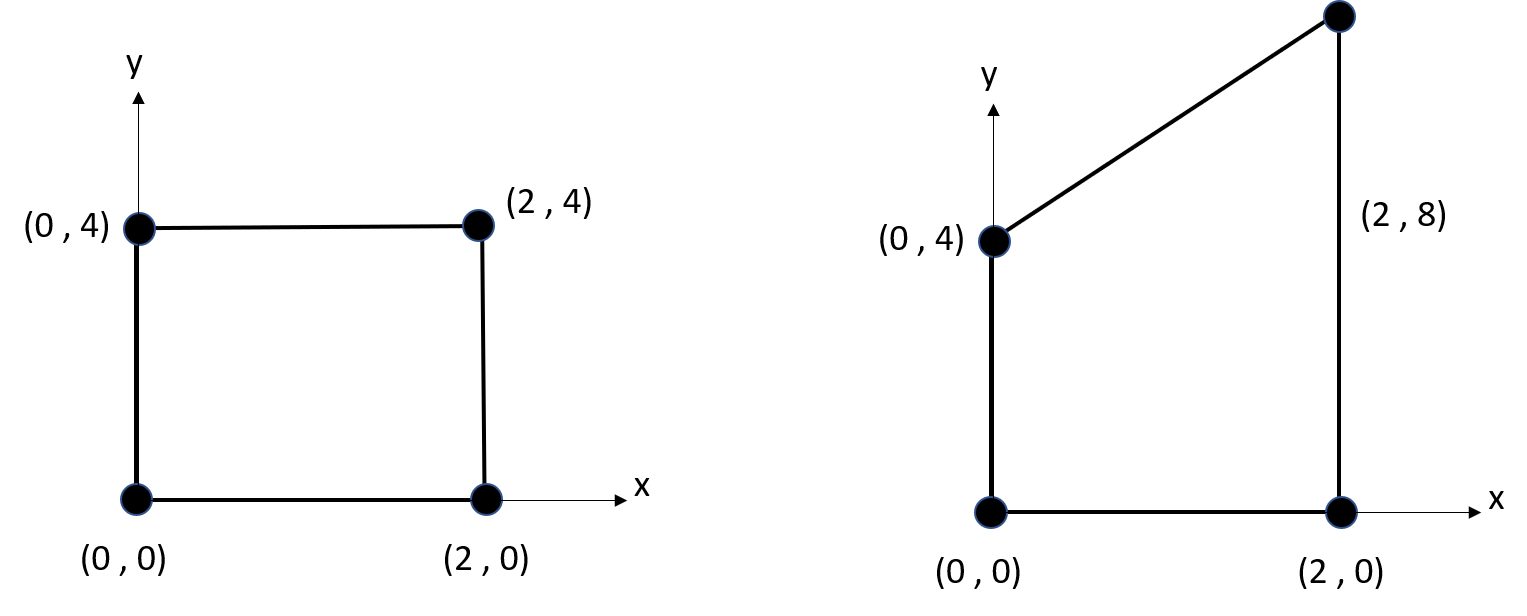
\includegraphics[width=0.65\textwidth]{domain1}
	\caption{Dominios de integración para el problema 1.}
	\label{fig:tan1}
\end{figure}

\item \label{punto02} Calcule la integral de la función
\[f(r,s)=rs\]
sobre el dominio triangular mostrado en la figura

\begin{figure}[H]
\centering
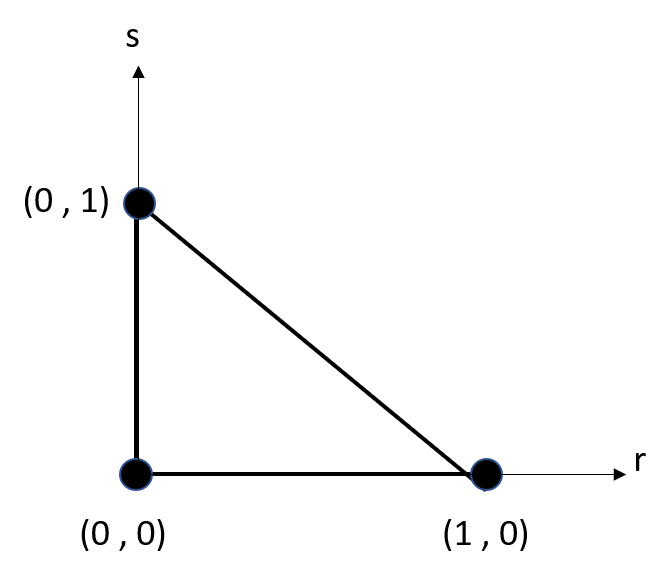
\includegraphics[width=0.50\textwidth]{domain3}
\caption{Dominios de integración para el problema 2.}
\label{fig:tan2}
\end{figure}
	
\item \label{punto03} Calcular las siguientes integrales usando una cuadratura 
de Gauss apropiada:
\begin{align*}
&I = \int_{1.0}^{1.5} x^2\ln x \dd{x} \\
&I = \int_0^\frac{\pi}{4} e^{3x} \sin2x\dd{x} \\
&I = \int_0^\frac{\pi}{4} \cos^2x\dd{x}
\end{align*}
	
\end{enumerate}
